\documentclass[a4paper]{book}
\usepackage{makeidx}
\usepackage{natbib}
\usepackage{graphicx}
\usepackage{multicol}
\usepackage{float}
\usepackage{listings}
\usepackage{color}
\usepackage{ifthen}
\usepackage[table]{xcolor}
\usepackage{textcomp}
\usepackage{alltt}
\usepackage{ifpdf}
\ifpdf
\usepackage[pdftex,
            pagebackref=true,
            colorlinks=true,
            linkcolor=blue,
            unicode
           ]{hyperref}
\else
\usepackage[ps2pdf,
            pagebackref=true,
            colorlinks=true,
            linkcolor=blue,
            unicode
           ]{hyperref}
\usepackage{pspicture}
\fi
\usepackage[utf8]{inputenc}
\usepackage{mathptmx}
\usepackage[scaled=.90]{helvet}
\usepackage{courier}
\usepackage{sectsty}
\usepackage[titles]{tocloft}
\usepackage{doxygen}
\lstset{language=C++,inputencoding=utf8,basicstyle=\footnotesize,breaklines=true,breakatwhitespace=true,tabsize=8,numbers=left }
\makeindex
\setcounter{tocdepth}{3}
\renewcommand{\footrulewidth}{0.4pt}
\renewcommand{\familydefault}{\sfdefault}
\hfuzz=15pt
\setlength{\emergencystretch}{15pt}
\hbadness=750
\tolerance=750
\begin{document}
\hypersetup{pageanchor=false,citecolor=blue}
\begin{titlepage}
\vspace*{7cm}
\begin{center}
{\Large \-Drekar \-Engine }\\
\vspace*{1cm}
{\large \-Generated by Doxygen 1.7.5.1}\\
\vspace*{0.5cm}
{\small Tue Aug 7 2012 20:05:22}\\
\end{center}
\end{titlepage}
\clearemptydoublepage
\pagenumbering{roman}
\tableofcontents
\clearemptydoublepage
\pagenumbering{arabic}
\hypersetup{pageanchor=true,citecolor=blue}
\chapter{\-Module \-Index}
\section{\-Modules}
\-Here is a list of all modules\-:\begin{DoxyCompactList}
\item \contentsline{section}{\-Core}{\pageref{group___core}}{}
\item \contentsline{section}{\-Data}{\pageref{group___data}}{}
\end{DoxyCompactList}

\chapter{\-Namespace \-Index}
\section{\-Namespace \-List}
\-Here is a list of all documented namespaces with brief descriptions\-:\begin{DoxyCompactList}
\item\contentsline{section}{\hyperlink{namespacedata}{data} \\*\-Namespace of all data that lives in memory }{\pageref{namespacedata}}{}
\item\contentsline{section}{\hyperlink{namespacede}{de} \\*\-Namespace of the engine }{\pageref{namespacede}}{}
\end{DoxyCompactList}

\chapter{\-Class \-Index}
\section{\-Class \-Hierarchy}
\-This inheritance list is sorted roughly, but not completely, alphabetically\-:\begin{DoxyCompactList}
\item \contentsline{section}{de\-:\-:\-A\-Screen}{\pageref{classde_1_1_a_screen}}{}
\item \contentsline{section}{de\-:\-:\-Counted\-Object$<$ \-T $>$}{\pageref{classde_1_1_counted_object}}{}
\item \contentsline{section}{de\-:\-:\-Counted\-Object$<$ \-A\-Component $>$}{\pageref{classde_1_1_counted_object}}{}
\begin{DoxyCompactList}
\item \contentsline{section}{de\-:\-:\-A\-Component}{\pageref{classde_1_1_a_component}}{}
\begin{DoxyCompactList}
\item \contentsline{section}{de\-:\-:component\-:\-:\-Camera}{\pageref{classde_1_1component_1_1_camera}}{}
\item \contentsline{section}{de\-:\-:component\-:\-:\-Transform}{\pageref{classde_1_1component_1_1_transform}}{}
\end{DoxyCompactList}
\end{DoxyCompactList}
\item \contentsline{section}{de\-:\-:\-Counted\-Object$<$ \-Game\-Object $>$}{\pageref{classde_1_1_counted_object}}{}
\begin{DoxyCompactList}
\item \contentsline{section}{de\-:\-:\-Game\-Object}{\pageref{classde_1_1_game_object}}{}
\end{DoxyCompactList}
\item \contentsline{section}{de\-:\-:\-Counted\-Object$<$ \-Mesh $>$}{\pageref{classde_1_1_counted_object}}{}
\begin{DoxyCompactList}
\item \contentsline{section}{de\-:\-:data\-:\-:\-Mesh}{\pageref{classde_1_1data_1_1_mesh}}{}
\end{DoxyCompactList}
\item \contentsline{section}{de\-:\-:\-Counted\-Object$<$ \-Program $>$}{\pageref{classde_1_1_counted_object}}{}
\begin{DoxyCompactList}
\item \contentsline{section}{de\-:\-:\-Program}{\pageref{classde_1_1_program}}{}
\end{DoxyCompactList}
\item \contentsline{section}{de\-:\-:\-Counted\-Object$<$ \-Shader $>$}{\pageref{classde_1_1_counted_object}}{}
\begin{DoxyCompactList}
\item \contentsline{section}{de\-:\-:data\-:\-:\-Shader}{\pageref{classde_1_1data_1_1_shader}}{}
\end{DoxyCompactList}
\item \contentsline{section}{de\-:\-:\-Debug}{\pageref{classde_1_1_debug}}{}
\item \contentsline{section}{de\-:\-:\-Engine}{\pageref{classde_1_1_engine}}{}
\end{DoxyCompactList}

\chapter{\-Class \-Index}
\section{\-Class \-List}
\-Here are the classes, structs, unions and interfaces with brief descriptions\-:\begin{DoxyCompactList}
\item\contentsline{section}{\hyperlink{classde_1_1_a_component}{de\-::\-A\-Component} }{\pageref{classde_1_1_a_component}}{}
\item\contentsline{section}{\hyperlink{classde_1_1_a_screen}{de\-::\-A\-Screen} \\*\-This class define a screen. \-Subclass this to define the screens needed for your game. \-A screen is composed of a tree of object (the scene), and a \-G\-U\-I \-Layer. \-Screen are pushed into the screen pile of the \hyperlink{classde_1_1_engine}{\-Engine}. the engine always render/update the screen at the top of the pile }{\pageref{classde_1_1_a_screen}}{}
\item\contentsline{section}{\hyperlink{classde_1_1component_1_1_camera}{de\-::component\-::\-Camera} }{\pageref{classde_1_1component_1_1_camera}}{}
\item\contentsline{section}{\hyperlink{classde_1_1_counted_object}{de\-::\-Counted\-Object$<$ T $>$} \\*\-This class is the base class allowing to count object. \-It take car of tracking the copy, and release the object once not referenced by nothing \-The child class must implement a public \char`\"{}release()\char`\"{} function that must clean the object (instead of the destructor) \-N\-O\-T\-E \-: the object is deleted each time, only the function release is called once the count reach zero }{\pageref{classde_1_1_counted_object}}{}
\item\contentsline{section}{\hyperlink{classde_1_1_debug}{de\-::\-Debug} }{\pageref{classde_1_1_debug}}{}
\item\contentsline{section}{\hyperlink{classde_1_1_engine}{de\-::\-Engine} \\*\-Main class driving the \hyperlink{classde_1_1_engine}{\-Engine} }{\pageref{classde_1_1_engine}}{}
\item\contentsline{section}{\hyperlink{classde_1_1_game_object}{de\-::\-Game\-Object} }{\pageref{classde_1_1_game_object}}{}
\item\contentsline{section}{\hyperlink{classde_1_1data_1_1_mesh}{de\-::data\-::\-Mesh} \\*\-Describe a \hyperlink{classde_1_1data_1_1_mesh}{\-Mesh} in memory }{\pageref{classde_1_1data_1_1_mesh}}{}
\item\contentsline{section}{\hyperlink{classde_1_1_program}{de\-::\-Program} }{\pageref{classde_1_1_program}}{}
\item\contentsline{section}{\hyperlink{classde_1_1data_1_1_shader}{de\-::data\-::\-Shader} \\*\-Encapsulate a shader. \-Simply allow simple loading from file }{\pageref{classde_1_1data_1_1_shader}}{}
\item\contentsline{section}{\hyperlink{classde_1_1component_1_1_transform}{de\-::component\-::\-Transform} }{\pageref{classde_1_1component_1_1_transform}}{}
\end{DoxyCompactList}

\chapter{\-Module \-Documentation}
\hypertarget{group___core}{
\section{\-Core}
\label{group___core}\index{\-Core@{\-Core}}
}


\-Core of the engine.  


\-Core of the engine. 
\hypertarget{group___data}{
\section{\-Data}
\label{group___data}\index{\-Data@{\-Data}}
}


\-Data that live in memory.  


\-Data that live in memory. \-All data that live in memory before being \char`\"{}used\char`\"{}, like mesh before being upload in \-V\-B\-O etc... 
\chapter{\-Namespace \-Documentation}
\hypertarget{namespacedata}{
\section{data \-Namespace \-Reference}
\label{namespacedata}\index{data@{data}}
}


the namespace of all data that lives in memory.  




\subsection{\-Detailed \-Description}
the namespace of all data that lives in memory. 
\hypertarget{namespacede}{
\section{de \-Namespace \-Reference}
\label{namespacede}\index{de@{de}}
}


the namespace of the engine  


\subsection*{\-Classes}
\begin{DoxyCompactItemize}
\item 
class \hyperlink{classde_1_1_a_component}{\-A\-Component}
\item 
class \hyperlink{classde_1_1_a_screen}{\-A\-Screen}
\begin{DoxyCompactList}\small\item\em \-This class define a screen. \-Subclass this to define the screens needed for your game. \-A screen is composed of a tree of object (the scene), and a \-G\-U\-I \-Layer. \-Screen are pushed into the screen pile of the \hyperlink{classde_1_1_engine}{\-Engine}. the engine always render/update the screen at the top of the pile. \end{DoxyCompactList}\item 
class \hyperlink{classde_1_1_counted_object}{\-Counted\-Object}
\begin{DoxyCompactList}\small\item\em this class is the base class allowing to count object. \-It take car of tracking the copy, and release the object once not referenced by nothing \-The child class must implement a public \char`\"{}release()\char`\"{} function that must clean the object (instead of the destructor) \-N\-O\-T\-E \-: the object is deleted each time, only the function release is called once the count reach zero. \end{DoxyCompactList}\item 
class \hyperlink{classde_1_1_debug}{\-Debug}
\item 
class \hyperlink{classde_1_1_engine}{\-Engine}
\begin{DoxyCompactList}\small\item\em \-Main class driving the \hyperlink{classde_1_1_engine}{\-Engine}. \end{DoxyCompactList}\item 
class \hyperlink{classde_1_1_game_object}{\-Game\-Object}
\item 
class \hyperlink{classde_1_1_program}{\-Program}
\end{DoxyCompactItemize}


\subsection{\-Detailed \-Description}
the namespace of the engine 
\chapter{\-Class \-Documentation}
\hypertarget{classde_1_1_a_component}{
\section{de\-:\-:\-A\-Component \-Class \-Reference}
\label{classde_1_1_a_component}\index{de\-::\-A\-Component@{de\-::\-A\-Component}}
}
\-Inheritance diagram for de\-:\-:\-A\-Component\-:\begin{figure}[H]
\begin{center}
\leavevmode
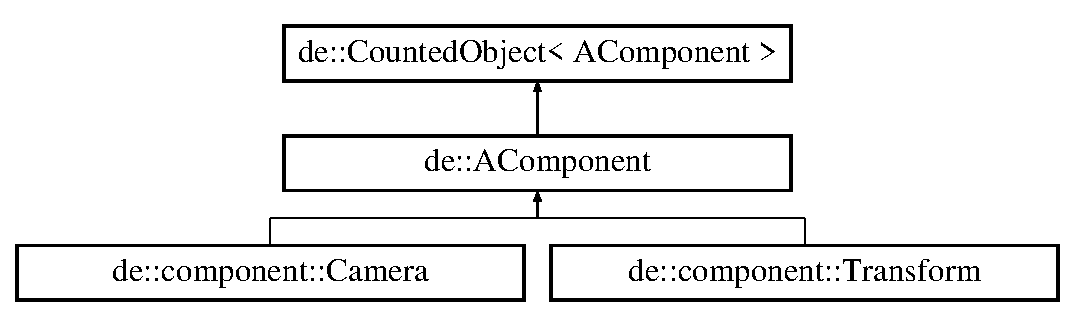
\includegraphics[height=3.000000cm]{classde_1_1_a_component}
\end{center}
\end{figure}
\subsection*{\-Public \-Member \-Functions}
\begin{DoxyCompactItemize}
\item 
\hypertarget{classde_1_1_a_component_a7ab24a42d85ff99b43e48b65f632945e}{
virtual void \hyperlink{classde_1_1_a_component_a7ab24a42d85ff99b43e48b65f632945e}{init} ()}
\label{classde_1_1_a_component_a7ab24a42d85ff99b43e48b65f632945e}

\begin{DoxyCompactList}\small\item\em called by the gameobject once the component has been had to its component list \end{DoxyCompactList}\item 
\hypertarget{classde_1_1_a_component_a21411259fcb39ed538cb4c0a2f48d0bd}{
virtual void \hyperlink{classde_1_1_a_component_a21411259fcb39ed538cb4c0a2f48d0bd}{update} ()}
\label{classde_1_1_a_component_a21411259fcb39ed538cb4c0a2f48d0bd}

\begin{DoxyCompactList}\small\item\em called each update \end{DoxyCompactList}\item 
\hypertarget{classde_1_1_a_component_a2f7e56f9d37db6cffff0aa3b5f86e346}{
virtual void \hyperlink{classde_1_1_a_component_a2f7e56f9d37db6cffff0aa3b5f86e346}{late\-Update} ()}
\label{classde_1_1_a_component_a2f7e56f9d37db6cffff0aa3b5f86e346}

\begin{DoxyCompactList}\small\item\em called after each update but before each draw \end{DoxyCompactList}\item 
\hypertarget{classde_1_1_a_component_ad1657f2e375354e70b94bbe86fae721b}{
virtual void \hyperlink{classde_1_1_a_component_ad1657f2e375354e70b94bbe86fae721b}{draw} ()}
\label{classde_1_1_a_component_ad1657f2e375354e70b94bbe86fae721b}

\begin{DoxyCompactList}\small\item\em called each draw \end{DoxyCompactList}\item 
\hypertarget{classde_1_1_a_component_a02ecbe18d2fa3449b66a59656a1040d5}{
void {\bfseries release} ()}
\label{classde_1_1_a_component_a02ecbe18d2fa3449b66a59656a1040d5}

\end{DoxyCompactItemize}
\subsection*{\-Protected \-Attributes}
\begin{DoxyCompactItemize}
\item 
\hypertarget{classde_1_1_a_component_a068c136424815a8b7b2026a5c4787de0}{
\hyperlink{classde_1_1_game_object}{\-Game\-Object} $\ast$ {\bfseries m\-Owner}}
\label{classde_1_1_a_component_a068c136424815a8b7b2026a5c4787de0}

\end{DoxyCompactItemize}
\subsection*{\-Friends}
\begin{DoxyCompactItemize}
\item 
\hypertarget{classde_1_1_a_component_a00df87c957d8f7ee0fc51f07a0542f4a}{
class {\bfseries \-Game\-Object}}
\label{classde_1_1_a_component_a00df87c957d8f7ee0fc51f07a0542f4a}

\end{DoxyCompactItemize}


\-The documentation for this class was generated from the following file\-:\begin{DoxyCompactItemize}
\item 
include/core/\-A\-Component.\-h\end{DoxyCompactItemize}

\hypertarget{classde_1_1_a_screen}{
\section{de\-:\-:\-A\-Screen \-Class \-Reference}
\label{classde_1_1_a_screen}\index{de\-::\-A\-Screen@{de\-::\-A\-Screen}}
}


\-This class define a screen. \-Subclass this to define the screens needed for your game. \-A screen is composed of a tree of object (the scene), and a \-G\-U\-I \-Layer. \-Screen are pushed into the screen pile of the \hyperlink{classde_1_1_engine}{\-Engine}. the engine always render/update the screen at the top of the pile.  




{\ttfamily \#include $<$\-A\-Screen.\-h$>$}

\subsection*{\-Public \-Member \-Functions}
\begin{DoxyCompactItemize}
\item 
\hypertarget{classde_1_1_a_screen_a28b840683b1ca50d0c983eb0456fe0e3}{
virtual void {\bfseries init} ()}
\label{classde_1_1_a_screen_a28b840683b1ca50d0c983eb0456fe0e3}

\item 
\hypertarget{classde_1_1_a_screen_a705a669f2e391475a5237d530cca09c8}{
virtual void \hyperlink{classde_1_1_a_screen_a705a669f2e391475a5237d530cca09c8}{update} ()}
\label{classde_1_1_a_screen_a705a669f2e391475a5237d530cca09c8}

\begin{DoxyCompactList}\small\item\em you \-H\-A\-V\-E to call this base class update in your sublcass, to allow updating of the internal of the engine \end{DoxyCompactList}\item 
\hypertarget{classde_1_1_a_screen_ad4e30171aeab1824fb60958cfa18ca8b}{
virtual void \hyperlink{classde_1_1_a_screen_ad4e30171aeab1824fb60958cfa18ca8b}{draw} ()}
\label{classde_1_1_a_screen_ad4e30171aeab1824fb60958cfa18ca8b}

\begin{DoxyCompactList}\small\item\em you \-H\-A\-V\-E to call this base class draw in your subclass, to allow drawing the scene tree. \end{DoxyCompactList}\end{DoxyCompactItemize}


\subsection{\-Detailed \-Description}
\-This class define a screen. \-Subclass this to define the screens needed for your game. \-A screen is composed of a tree of object (the scene), and a \-G\-U\-I \-Layer. \-Screen are pushed into the screen pile of the \hyperlink{classde_1_1_engine}{\-Engine}. the engine always render/update the screen at the top of the pile. 

\-The documentation for this class was generated from the following file\-:\begin{DoxyCompactItemize}
\item 
include/core/\-A\-Screen.\-h\end{DoxyCompactItemize}

\hypertarget{classde_1_1component_1_1_camera}{
\section{de\-:\-:component\-:\-:\-Camera \-Class \-Reference}
\label{classde_1_1component_1_1_camera}\index{de\-::component\-::\-Camera@{de\-::component\-::\-Camera}}
}
\-Inheritance diagram for de\-:\-:component\-:\-:\-Camera\-:\begin{figure}[H]
\begin{center}
\leavevmode
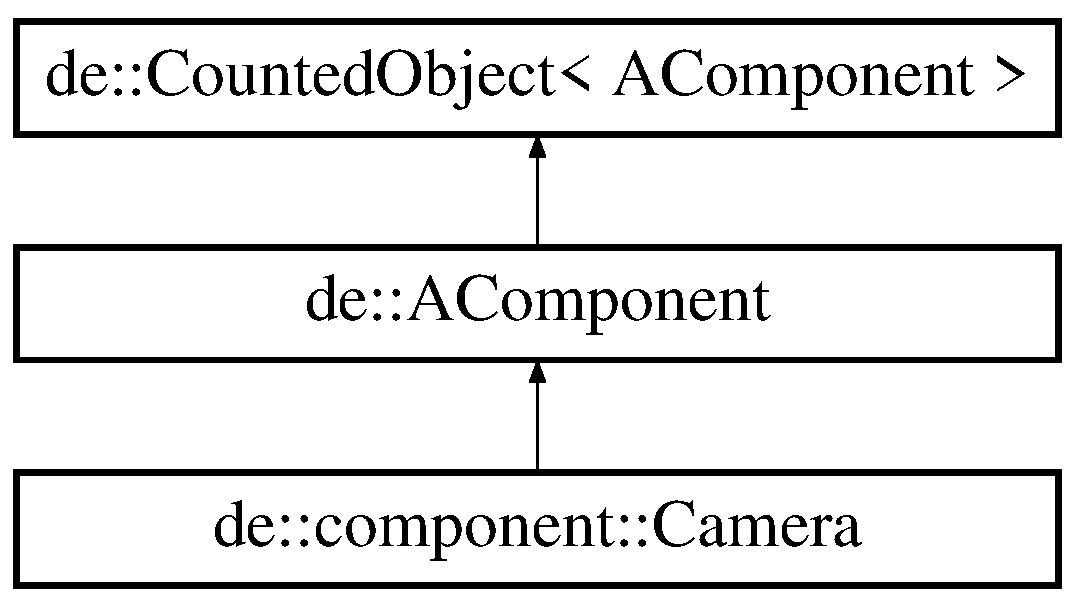
\includegraphics[height=3.000000cm]{classde_1_1component_1_1_camera}
\end{center}
\end{figure}
\subsection*{\-Public \-Member \-Functions}
\begin{DoxyCompactItemize}
\item 
\hypertarget{classde_1_1component_1_1_camera_a2ef98cdce449ec142368b235bd235e5b}{
void \hyperlink{classde_1_1component_1_1_camera_a2ef98cdce449ec142368b235bd235e5b}{init} ()}
\label{classde_1_1component_1_1_camera_a2ef98cdce449ec142368b235bd235e5b}

\begin{DoxyCompactList}\small\item\em called by the gameobject once the component has been had to its component list \end{DoxyCompactList}\item 
\hypertarget{classde_1_1component_1_1_camera_a2f014c4f6467735c3e527f26fbb95c90}{
void \hyperlink{classde_1_1component_1_1_camera_a2f014c4f6467735c3e527f26fbb95c90}{update} ()}
\label{classde_1_1component_1_1_camera_a2f014c4f6467735c3e527f26fbb95c90}

\begin{DoxyCompactList}\small\item\em called each update \end{DoxyCompactList}\item 
\hypertarget{classde_1_1component_1_1_camera_a3d5829322081062984cfef94f4ac4f14}{
void {\bfseries set\-Fov} (float p\-Fov)}
\label{classde_1_1component_1_1_camera_a3d5829322081062984cfef94f4ac4f14}

\item 
\hypertarget{classde_1_1component_1_1_camera_af5579f5f972add9e50cd112678c67445}{
void {\bfseries set\-Aspect} (float p\-Aspect)}
\label{classde_1_1component_1_1_camera_af5579f5f972add9e50cd112678c67445}

\item 
\hypertarget{classde_1_1component_1_1_camera_a798de6d6cc71f7102937e98e4c06fd9c}{
void {\bfseries set\-Clip\-Plane} (glm\-::vec2 \&p\-Clip\-Plane)}
\label{classde_1_1component_1_1_camera_a798de6d6cc71f7102937e98e4c06fd9c}

\end{DoxyCompactItemize}
\subsection*{\-Protected \-Member \-Functions}
\begin{DoxyCompactItemize}
\item 
\hypertarget{classde_1_1component_1_1_camera_a86423dc08e6d56abeea66fc805d43048}{
void {\bfseries compute\-Projection} ()}
\label{classde_1_1component_1_1_camera_a86423dc08e6d56abeea66fc805d43048}

\end{DoxyCompactItemize}
\subsection*{\-Protected \-Attributes}
\begin{DoxyCompactItemize}
\item 
\hypertarget{classde_1_1component_1_1_camera_a8c5f7fd5ffae706186dbf03a048bdc5d}{
std\-::list$<$ \hyperlink{classde_1_1component_1_1_camera}{\-Camera} $\ast$ $>$ {\bfseries s\-Camera\-List}}
\label{classde_1_1component_1_1_camera_a8c5f7fd5ffae706186dbf03a048bdc5d}

\item 
\hypertarget{classde_1_1component_1_1_camera_a2b7327497effbec1fb121b6c3cbb8573}{
glm\-::mat4 {\bfseries m\-Projection}}
\label{classde_1_1component_1_1_camera_a2b7327497effbec1fb121b6c3cbb8573}

\item 
\hypertarget{classde_1_1component_1_1_camera_ad05c34679985bb26b81fc42d90ad0efb}{
float {\bfseries m\-Fov}}
\label{classde_1_1component_1_1_camera_ad05c34679985bb26b81fc42d90ad0efb}

\item 
\hypertarget{classde_1_1component_1_1_camera_a21555a64ca5dfeb1e9bcc5e34be934cf}{
float {\bfseries m\-Aspect}}
\label{classde_1_1component_1_1_camera_a21555a64ca5dfeb1e9bcc5e34be934cf}

\item 
\hypertarget{classde_1_1component_1_1_camera_ace8f2bcca61e08b2d6e4b2863d367c54}{
glm\-::vec2 {\bfseries m\-Clip\-Planes}}
\label{classde_1_1component_1_1_camera_ace8f2bcca61e08b2d6e4b2863d367c54}

\item 
\hypertarget{classde_1_1component_1_1_camera_a4f47596f8d746b39940afa43c68f6512}{
bool {\bfseries m\-Recompute\-Projecton}}
\label{classde_1_1component_1_1_camera_a4f47596f8d746b39940afa43c68f6512}

\end{DoxyCompactItemize}


\-The documentation for this class was generated from the following file\-:\begin{DoxyCompactItemize}
\item 
include/component/\-Camera.\-h\end{DoxyCompactItemize}

\hypertarget{classde_1_1_counted_object}{
\section{de\-:\-:\-Counted\-Object$<$ \-T $>$ \-Class \-Template \-Reference}
\label{classde_1_1_counted_object}\index{de\-::\-Counted\-Object$<$ T $>$@{de\-::\-Counted\-Object$<$ T $>$}}
}


this class is the base class allowing to count object. \-It take car of tracking the copy, and release the object once not referenced by nothing \-The child class must implement a public \char`\"{}release()\char`\"{} function that must clean the object (instead of the destructor) \-N\-O\-T\-E \-: the object is deleted each time, only the function release is called once the count reach zero.  




{\ttfamily \#include $<$\-Counted\-Object.\-h$>$}

\subsection*{\-Public \-Member \-Functions}
\begin{DoxyCompactItemize}
\item 
\hypertarget{classde_1_1_counted_object_a6f5d16c74555894b096f354625b4d903}{
{\bfseries \-Counted\-Object} (const \hyperlink{classde_1_1_counted_object}{\-Counted\-Object} \&p\-Other)}
\label{classde_1_1_counted_object_a6f5d16c74555894b096f354625b4d903}

\item 
\hypertarget{classde_1_1_counted_object_a0fd6acfd589acd511c81934f025980c9}{
\hyperlink{classde_1_1_counted_object}{\-Counted\-Object} \& {\bfseries operator=} (const \hyperlink{classde_1_1_counted_object}{\-Counted\-Object} \&p\-Other)}
\label{classde_1_1_counted_object_a0fd6acfd589acd511c81934f025980c9}

\end{DoxyCompactItemize}
\subsection*{\-Protected \-Attributes}
\begin{DoxyCompactItemize}
\item 
\hypertarget{classde_1_1_counted_object_acb48eadb2bf07a7eb0d5e1d8eff795c8}{
int $\ast$ {\bfseries m\-Numbers}}
\label{classde_1_1_counted_object_acb48eadb2bf07a7eb0d5e1d8eff795c8}

\end{DoxyCompactItemize}


\subsection{\-Detailed \-Description}
\subsubsection*{template$<$class \-T$>$class de\-::\-Counted\-Object$<$ T $>$}

this class is the base class allowing to count object. \-It take car of tracking the copy, and release the object once not referenced by nothing \-The child class must implement a public \char`\"{}release()\char`\"{} function that must clean the object (instead of the destructor) \-N\-O\-T\-E \-: the object is deleted each time, only the function release is called once the count reach zero. 

\-The documentation for this class was generated from the following file\-:\begin{DoxyCompactItemize}
\item 
include/core/\-Counted\-Object.\-h\end{DoxyCompactItemize}

\hypertarget{classde_1_1_debug}{
\section{de\-:\-:\-Debug \-Class \-Reference}
\label{classde_1_1_debug}\index{de\-::\-Debug@{de\-::\-Debug}}
}
\subsection*{\-Static \-Public \-Member \-Functions}
\begin{DoxyCompactItemize}
\item 
\hypertarget{classde_1_1_debug_a87d49a56764c788a9e563f90a5755301}{
static void {\bfseries \-Log} (std\-::string p\-Info)}
\label{classde_1_1_debug_a87d49a56764c788a9e563f90a5755301}

\end{DoxyCompactItemize}
\subsection*{\-Protected \-Attributes}
\begin{DoxyCompactItemize}
\item 
\hypertarget{classde_1_1_debug_a0db959b3bc57df16fdf0fcd47daa291b}{
std\-::string {\bfseries m\-Path}}
\label{classde_1_1_debug_a0db959b3bc57df16fdf0fcd47daa291b}

\end{DoxyCompactItemize}
\subsection*{\-Static \-Protected \-Attributes}
\begin{DoxyCompactItemize}
\item 
\hypertarget{classde_1_1_debug_acd5e31a4a54fc528dfdc202d36c0c7ac}{
static \hyperlink{classde_1_1_debug}{\-Debug} $\ast$ {\bfseries s\-Instance}}
\label{classde_1_1_debug_acd5e31a4a54fc528dfdc202d36c0c7ac}

\end{DoxyCompactItemize}


\-The documentation for this class was generated from the following file\-:\begin{DoxyCompactItemize}
\item 
include/core/\-Debug.\-h\end{DoxyCompactItemize}

\hypertarget{classde_1_1_engine}{
\section{de\-:\-:\-Engine \-Class \-Reference}
\label{classde_1_1_engine}\index{de\-::\-Engine@{de\-::\-Engine}}
}


\-Main class driving the \hyperlink{classde_1_1_engine}{\-Engine}.  




{\ttfamily \#include $<$\-Engine.\-h$>$}

\subsection*{\-Static \-Public \-Member \-Functions}
\begin{DoxyCompactItemize}
\item 
\hypertarget{classde_1_1_engine_ac4c2011633fe02a8d501b4a44c24d9c6}{
static void {\bfseries initialize} (int p\-Width=800, int p\-Height=600, bool p\-Fullscreen=false)}
\label{classde_1_1_engine_ac4c2011633fe02a8d501b4a44c24d9c6}

\item 
\hypertarget{classde_1_1_engine_afe7222c75b761a87e97755b25012a155}{
static void {\bfseries loop} ()}
\label{classde_1_1_engine_afe7222c75b761a87e97755b25012a155}

\item 
\hypertarget{classde_1_1_engine_a560c70eb0a07fc209672ebd0be8b3bc6}{
static void \hyperlink{classde_1_1_engine_a560c70eb0a07fc209672ebd0be8b3bc6}{push\-Screen} (\hyperlink{classde_1_1_a_screen}{\-A\-Screen} $\ast$p\-Screen)}
\label{classde_1_1_engine_a560c70eb0a07fc209672ebd0be8b3bc6}

\begin{DoxyCompactList}\small\item\em push a screen on the pile, it became the new updated/rendered screen \end{DoxyCompactList}\item 
\hypertarget{classde_1_1_engine_a52230fb1aedeef894a1e5adfe0923d57}{
static \hyperlink{classde_1_1_a_screen}{\-A\-Screen} $\ast$ \hyperlink{classde_1_1_engine_a52230fb1aedeef894a1e5adfe0923d57}{pop\-Screen} ()}
\label{classde_1_1_engine_a52230fb1aedeef894a1e5adfe0923d57}

\begin{DoxyCompactList}\small\item\em pop the screen from the pile and return it. if you wish to delete the screen pass true as argument, this will flag the screen for deletion. \-Avoid deleting the screen right away, especialy if it's the current main screen... \end{DoxyCompactList}\end{DoxyCompactItemize}
\subsection*{\-Protected \-Member \-Functions}
\begin{DoxyCompactItemize}
\item 
\hypertarget{classde_1_1_engine_a9263c32f13aa37f5cc5d747b21b3c891}{
{\bfseries \-Engine} (int p\-Width, int p\-Height, bool p\-Fullscreen)}
\label{classde_1_1_engine_a9263c32f13aa37f5cc5d747b21b3c891}

\end{DoxyCompactItemize}
\subsection*{\-Protected \-Attributes}
\begin{DoxyCompactItemize}
\item 
\hypertarget{classde_1_1_engine_abaf67500a242fdcbe850d0c45ee30636}{
int {\bfseries m\-Width}}
\label{classde_1_1_engine_abaf67500a242fdcbe850d0c45ee30636}

\item 
\hypertarget{classde_1_1_engine_a9fe6e8f5b32ed72b76e1194bab99feb1}{
int {\bfseries m\-Height}}
\label{classde_1_1_engine_a9fe6e8f5b32ed72b76e1194bab99feb1}

\item 
\hypertarget{classde_1_1_engine_a335a0392ce9cfc6ce5625ea991d4849d}{
bool {\bfseries m\-Fullscreen}}
\label{classde_1_1_engine_a335a0392ce9cfc6ce5625ea991d4849d}

\item 
\hypertarget{classde_1_1_engine_ac9af7310cc233aa5dd2149e7f6dfe6c6}{
bool {\bfseries m\-Running}}
\label{classde_1_1_engine_ac9af7310cc233aa5dd2149e7f6dfe6c6}

\item 
\hypertarget{classde_1_1_engine_af81f599248b3a98783e4250b57f180b9}{
std\-::list$<$ \hyperlink{classde_1_1_a_screen}{\-A\-Screen} $\ast$ $>$ {\bfseries m\-Screens}}
\label{classde_1_1_engine_af81f599248b3a98783e4250b57f180b9}

\item 
\hypertarget{classde_1_1_engine_a328645ef9103750ac2bc24b4ddd7963c}{
std\-::list$<$ \hyperlink{classde_1_1_a_screen}{\-A\-Screen} $\ast$ $>$ {\bfseries m\-Init\-Screens}}
\label{classde_1_1_engine_a328645ef9103750ac2bc24b4ddd7963c}

\item 
\hypertarget{classde_1_1_engine_a9629a734c18b2d077c42df1398090735}{
std\-::list$<$ \hyperlink{classde_1_1_a_screen}{\-A\-Screen} $\ast$ $>$ {\bfseries m\-Delete\-Screens}}
\label{classde_1_1_engine_a9629a734c18b2d077c42df1398090735}

\end{DoxyCompactItemize}
\subsection*{\-Static \-Protected \-Attributes}
\begin{DoxyCompactItemize}
\item 
\hypertarget{classde_1_1_engine_a582339f67689e2e5f799f37017454282}{
static \hyperlink{classde_1_1_engine}{\-Engine} $\ast$ {\bfseries s\-Instance}}
\label{classde_1_1_engine_a582339f67689e2e5f799f37017454282}

\end{DoxyCompactItemize}


\subsection{\-Detailed \-Description}
\-Main class driving the \hyperlink{classde_1_1_engine}{\-Engine}. 

\-This class cannot be instantiated. \-Instead initialize should be used. \-All the interface is throught static method, a simple use would be


\begin{DoxyCode}
     Engine::initialize(800, 600, false);
     Engine::loop();//launch the rendering loop, that will call update/draw on
       all screens
\end{DoxyCode}
 

\-The documentation for this class was generated from the following file\-:\begin{DoxyCompactItemize}
\item 
include/core/\-Engine.\-h\end{DoxyCompactItemize}

\hypertarget{classde_1_1_game_object}{
\section{de\-:\-:\-Game\-Object \-Class \-Reference}
\label{classde_1_1_game_object}\index{de\-::\-Game\-Object@{de\-::\-Game\-Object}}
}
\-Inheritance diagram for de\-:\-:\-Game\-Object\-:\begin{figure}[H]
\begin{center}
\leavevmode
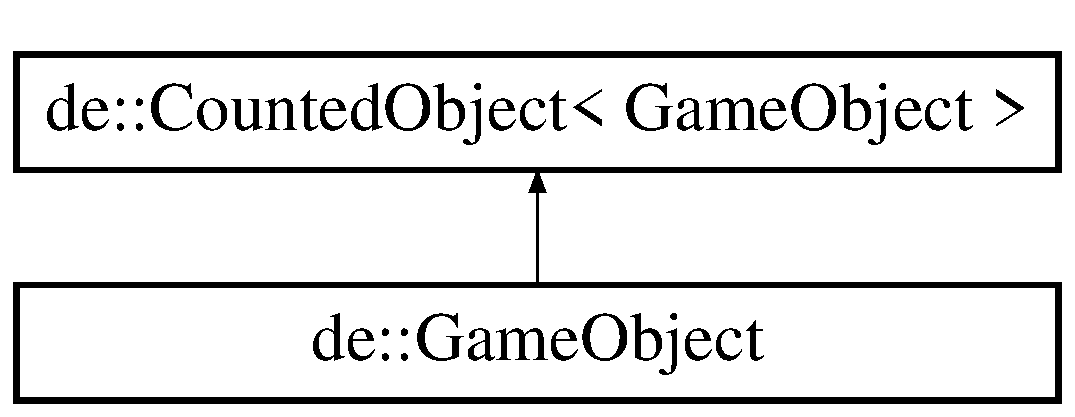
\includegraphics[height=2.000000cm]{classde_1_1_game_object}
\end{center}
\end{figure}
\subsection*{\-Public \-Member \-Functions}
\begin{DoxyCompactItemize}
\item 
\hypertarget{classde_1_1_game_object_a68be8d3d6c07b8ffddb22b7758a36b51}{
{\bfseries \-Game\-Object} (std\-::string p\-Name)}
\label{classde_1_1_game_object_a68be8d3d6c07b8ffddb22b7758a36b51}

\item 
\hypertarget{classde_1_1_game_object_a7cf452c9ec1ad16d2f45d493f51974a7}{
void {\bfseries release} ()}
\label{classde_1_1_game_object_a7cf452c9ec1ad16d2f45d493f51974a7}

\item 
\hypertarget{classde_1_1_game_object_adaa68cb3c475ade540ab527543210096}{
virtual void \hyperlink{classde_1_1_game_object_adaa68cb3c475ade540ab527543210096}{update} ()}
\label{classde_1_1_game_object_adaa68cb3c475ade540ab527543210096}

\begin{DoxyCompactList}\small\item\em override this to implement per-\/frame behavior. \-It's called before interal\-Update, mean that component get updated \-A\-F\-T\-E\-R this. \-This allow to modify their values and see this repercuted this frame.) \end{DoxyCompactList}\item 
\hypertarget{classde_1_1_game_object_a7530cc647d3c51516a710dd91cc99c09}{
virtual void \hyperlink{classde_1_1_game_object_a7530cc647d3c51516a710dd91cc99c09}{draw} ()}
\label{classde_1_1_game_object_a7530cc647d3c51516a710dd91cc99c09}

\begin{DoxyCompactList}\small\item\em override this to define a behaviour just before drawing \end{DoxyCompactList}\item 
\hypertarget{classde_1_1_game_object_a113db17ce4217a18053e4125a936eb41}{
\hyperlink{classde_1_1_a_component}{\-A\-Component} $\ast$ \hyperlink{classde_1_1_game_object_a113db17ce4217a18053e4125a936eb41}{add\-Component} (\hyperlink{classde_1_1_a_component}{\-A\-Component} $\ast$p\-Component)}
\label{classde_1_1_game_object_a113db17ce4217a18053e4125a936eb41}

\begin{DoxyCompactList}\small\item\em add a component to the gameobject return the component passed as argument for chaining \end{DoxyCompactList}\item 
\hypertarget{classde_1_1_game_object_a6f25a7fe1d2ec1ae206a8dc52733a4d6}{
\hyperlink{classde_1_1component_1_1_transform}{component\-::\-Transform} $\ast$ \hyperlink{classde_1_1_game_object_a6f25a7fe1d2ec1ae206a8dc52733a4d6}{transform} ()}
\label{classde_1_1_game_object_a6f25a7fe1d2ec1ae206a8dc52733a4d6}

\begin{DoxyCompactList}\small\item\em simply a shortcut to the transform component of this \hyperlink{classde_1_1_game_object}{\-Game\-Object} \end{DoxyCompactList}\end{DoxyCompactItemize}
\subsection*{\-Protected \-Attributes}
\begin{DoxyCompactItemize}
\item 
\hypertarget{classde_1_1_game_object_a946fc91be8a39c450f985d8852f3ed02}{
\hyperlink{classde_1_1_game_object}{\-Game\-Object} $\ast$ {\bfseries m\-Parent}}
\label{classde_1_1_game_object_a946fc91be8a39c450f985d8852f3ed02}

\item 
\hypertarget{classde_1_1_game_object_a1faf0cb425332b0d252dad8082089fd8}{
std\-::list$<$ \hyperlink{classde_1_1_game_object}{\-Game\-Object} $\ast$ $>$ {\bfseries m\-Children}}
\label{classde_1_1_game_object_a1faf0cb425332b0d252dad8082089fd8}

\item 
\hypertarget{classde_1_1_game_object_a1d5028e8aef6e3643d834fdfc555db61}{
std\-::list$<$ \hyperlink{classde_1_1_a_component}{\-A\-Component} $\ast$ $>$ {\bfseries m\-Components}}
\label{classde_1_1_game_object_a1d5028e8aef6e3643d834fdfc555db61}

\item 
\hypertarget{classde_1_1_game_object_a4e0cccd0d009116e04fd92cc3d746a33}{
\hyperlink{classde_1_1component_1_1_transform}{component\-::\-Transform} $\ast$ {\bfseries m\-Transform}}
\label{classde_1_1_game_object_a4e0cccd0d009116e04fd92cc3d746a33}

\end{DoxyCompactItemize}
\subsection*{\-Friends}
\begin{DoxyCompactItemize}
\item 
\hypertarget{classde_1_1_game_object_ae1b9dd8d05ef01c165957ca5bbf66e72}{
class {\bfseries \-A\-Screen}}
\label{classde_1_1_game_object_ae1b9dd8d05ef01c165957ca5bbf66e72}

\end{DoxyCompactItemize}


\-The documentation for this class was generated from the following file\-:\begin{DoxyCompactItemize}
\item 
include/core/\-Gameobject.\-h\end{DoxyCompactItemize}

\hypertarget{classde_1_1data_1_1_mesh}{
\section{de\-:\-:data\-:\-:\-Mesh \-Class \-Reference}
\label{classde_1_1data_1_1_mesh}\index{de\-::data\-::\-Mesh@{de\-::data\-::\-Mesh}}
}


describe a \hyperlink{classde_1_1data_1_1_mesh}{\-Mesh} in memory  




{\ttfamily \#include $<$\-Mesh.\-h$>$}

\-Inheritance diagram for de\-:\-:data\-:\-:\-Mesh\-:\begin{figure}[H]
\begin{center}
\leavevmode
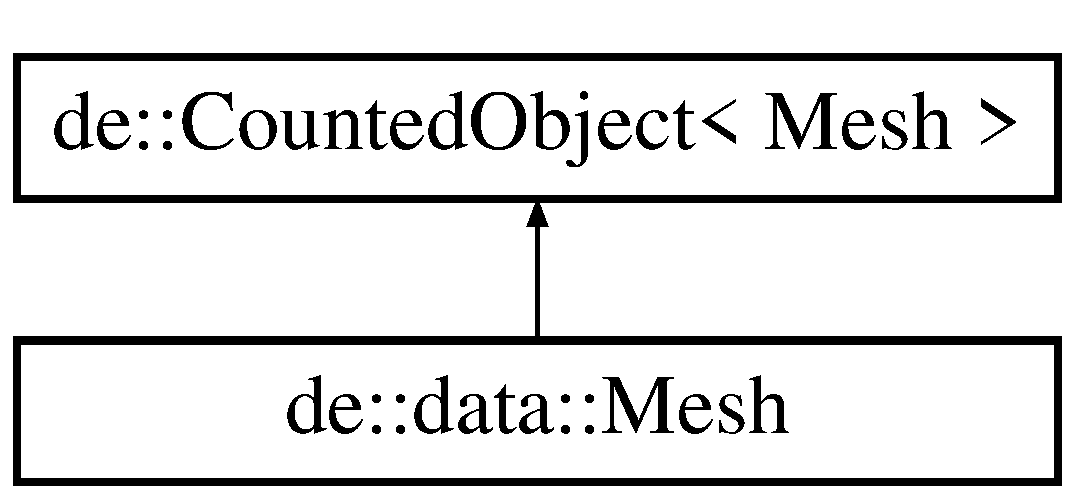
\includegraphics[height=2.000000cm]{classde_1_1data_1_1_mesh}
\end{center}
\end{figure}
\subsection*{\-Public \-Member \-Functions}
\begin{DoxyCompactItemize}
\item 
\hypertarget{classde_1_1data_1_1_mesh_addb8861b2351da42135689571264ee04}{
{\bfseries \-Mesh} (std\-::string p\-Path)}
\label{classde_1_1data_1_1_mesh_addb8861b2351da42135689571264ee04}

\item 
\hypertarget{classde_1_1data_1_1_mesh_a3fed7c0c97c9ec90cf5492ddf004ad1f}{
void {\bfseries release} ()}
\label{classde_1_1data_1_1_mesh_a3fed7c0c97c9ec90cf5492ddf004ad1f}

\item 
\hypertarget{classde_1_1data_1_1_mesh_a839129c4498eeed6fec0c7a8f2fd37b7}{
void {\bfseries set\-Vertex} (glm\-::vec3 $\ast$p\-Vertex, unsigned int p\-Nb)}
\label{classde_1_1data_1_1_mesh_a839129c4498eeed6fec0c7a8f2fd37b7}

\item 
\hypertarget{classde_1_1data_1_1_mesh_a36ad426209872f9f20ad1dcbdc1bab5b}{
void {\bfseries set\-U\-V} (glm\-::vec2 $\ast$p\-Uv)}
\label{classde_1_1data_1_1_mesh_a36ad426209872f9f20ad1dcbdc1bab5b}

\item 
\hypertarget{classde_1_1data_1_1_mesh_a37d002f94e2bbc71cc429f998ea6f308}{
void {\bfseries set\-Normal} (glm\-::vec3 $\ast$p\-Normal)}
\label{classde_1_1data_1_1_mesh_a37d002f94e2bbc71cc429f998ea6f308}

\item 
\hypertarget{classde_1_1data_1_1_mesh_ad837f307026269a13fe7dff0ed6b4c1c}{
void {\bfseries set\-Triangles} (int $\ast$p\-Triangles)}
\label{classde_1_1data_1_1_mesh_ad837f307026269a13fe7dff0ed6b4c1c}

\item 
\hypertarget{classde_1_1data_1_1_mesh_a5cd5aa76a532398e63aca29042dce0e1}{
void {\bfseries upload\-To\-V\-R\-A\-M} ()}
\label{classde_1_1data_1_1_mesh_a5cd5aa76a532398e63aca29042dce0e1}

\item 
\hypertarget{classde_1_1data_1_1_mesh_a7b8548c48d672c9bc085ecd906498e33}{
void {\bfseries draw} ()}
\label{classde_1_1data_1_1_mesh_a7b8548c48d672c9bc085ecd906498e33}

\end{DoxyCompactItemize}
\subsection*{\-Protected \-Attributes}
\begin{DoxyCompactItemize}
\item 
\hypertarget{classde_1_1data_1_1_mesh_aaf7d203e50bc556bdfac1e7222a9f199}{
int {\bfseries m\-Nb\-Vertex}}
\label{classde_1_1data_1_1_mesh_aaf7d203e50bc556bdfac1e7222a9f199}

\item 
\hypertarget{classde_1_1data_1_1_mesh_ae9dfb01b5452dadb9f6398f0b53e9f7d}{
glm\-::vec3 $\ast$ {\bfseries m\-Vertex}}
\label{classde_1_1data_1_1_mesh_ae9dfb01b5452dadb9f6398f0b53e9f7d}

\item 
\hypertarget{classde_1_1data_1_1_mesh_a4c6bbbf777959b963e7bfc24838e78df}{
glm\-::vec2 $\ast$ {\bfseries m\-Uvs}}
\label{classde_1_1data_1_1_mesh_a4c6bbbf777959b963e7bfc24838e78df}

\item 
\hypertarget{classde_1_1data_1_1_mesh_abc3e63ff9f0a159685f556aa87ce5762}{
glm\-::vec3 $\ast$ {\bfseries m\-Normals}}
\label{classde_1_1data_1_1_mesh_abc3e63ff9f0a159685f556aa87ce5762}

\item 
\hypertarget{classde_1_1data_1_1_mesh_a6f24ff8a3176033e6a09917a405db02d}{
glm\-::vec3 $\ast$ {\bfseries m\-Tangents}}
\label{classde_1_1data_1_1_mesh_a6f24ff8a3176033e6a09917a405db02d}

\item 
\hypertarget{classde_1_1data_1_1_mesh_af7522383c4508f0a82b27690fb36335d}{
int $\ast$ {\bfseries m\-Triangles}}
\label{classde_1_1data_1_1_mesh_af7522383c4508f0a82b27690fb36335d}

\item 
\hypertarget{classde_1_1data_1_1_mesh_ac35a2fe325686b438b09430cf827e9fe}{
\-G\-Luint {\bfseries m\-Open\-G\-L\-I\-D} \mbox{[}4\mbox{]}}
\label{classde_1_1data_1_1_mesh_ac35a2fe325686b438b09430cf827e9fe}

\end{DoxyCompactItemize}


\subsection{\-Detailed \-Description}
describe a \hyperlink{classde_1_1data_1_1_mesh}{\-Mesh} in memory 

\-The documentation for this class was generated from the following file\-:\begin{DoxyCompactItemize}
\item 
include/data/\-Mesh.\-h\end{DoxyCompactItemize}

\hypertarget{classde_1_1_program}{
\section{de\-:\-:\-Program \-Class \-Reference}
\label{classde_1_1_program}\index{de\-::\-Program@{de\-::\-Program}}
}
\-Inheritance diagram for de\-:\-:\-Program\-:\begin{figure}[H]
\begin{center}
\leavevmode
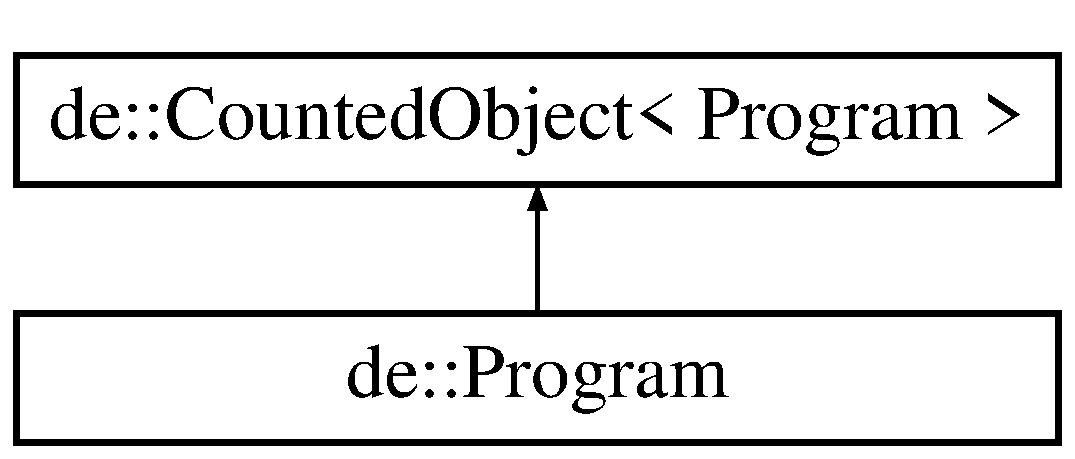
\includegraphics[height=2.000000cm]{classde_1_1_program}
\end{center}
\end{figure}
\subsection*{\-Public \-Member \-Functions}
\begin{DoxyCompactItemize}
\item 
\hypertarget{classde_1_1_program_ab63d578e8dcbf23be8e8772ae7ae33cb}{
void {\bfseries release} ()}
\label{classde_1_1_program_ab63d578e8dcbf23be8e8772ae7ae33cb}

\item 
\hypertarget{classde_1_1_program_a2dbfa8f7c448de8753e2a07cb67382cf}{
bool {\bfseries add\-Shader} (const \hyperlink{classde_1_1data_1_1_shader}{data\-::\-Shader} \&p\-Shader)}
\label{classde_1_1_program_a2dbfa8f7c448de8753e2a07cb67382cf}

\item 
\hypertarget{classde_1_1_program_a2f4c3aac6f60ceaab0f9cac3ccef51cc}{
bool {\bfseries compile} ()}
\label{classde_1_1_program_a2f4c3aac6f60ceaab0f9cac3ccef51cc}

\item 
\hypertarget{classde_1_1_program_a75bb5fe46cae5e1430b16da5ce2005c4}{
void {\bfseries set\-Matrix} (const std\-::string \&p\-Name, const glm\-::mat4 \&p\-Matrix)}
\label{classde_1_1_program_a75bb5fe46cae5e1430b16da5ce2005c4}

\item 
\hypertarget{classde_1_1_program_aec7c8cae5fea055b26b40299655a1b94}{
void {\bfseries use} ()}
\label{classde_1_1_program_aec7c8cae5fea055b26b40299655a1b94}

\end{DoxyCompactItemize}
\subsection*{\-Protected \-Attributes}
\begin{DoxyCompactItemize}
\item 
\hypertarget{classde_1_1_program_a6a86a66742d97071ff91487f785bd83c}{
int {\bfseries m\-I\-D}}
\label{classde_1_1_program_a6a86a66742d97071ff91487f785bd83c}

\item 
\hypertarget{classde_1_1_program_ab6272696655327867ed8c767365f8bda}{
bool {\bfseries m\-Linked}}
\label{classde_1_1_program_ab6272696655327867ed8c767365f8bda}

\item 
\hypertarget{classde_1_1_program_a42d4834609189072d28ac6d6dfeb75a5}{
std\-::map$<$ std\-::string, int $>$ {\bfseries m\-Uniforms}}
\label{classde_1_1_program_a42d4834609189072d28ac6d6dfeb75a5}

\end{DoxyCompactItemize}


\-The documentation for this class was generated from the following file\-:\begin{DoxyCompactItemize}
\item 
include/core/\-Program.\-h\end{DoxyCompactItemize}

\hypertarget{classde_1_1data_1_1_shader}{
\section{de\-:\-:data\-:\-:\-Shader \-Class \-Reference}
\label{classde_1_1data_1_1_shader}\index{de\-::data\-::\-Shader@{de\-::data\-::\-Shader}}
}


\-Encapsulate a shader. \-Simply allow simple loading from file.  




{\ttfamily \#include $<$\-Shader.\-h$>$}

\-Inheritance diagram for de\-:\-:data\-:\-:\-Shader\-:\begin{figure}[H]
\begin{center}
\leavevmode
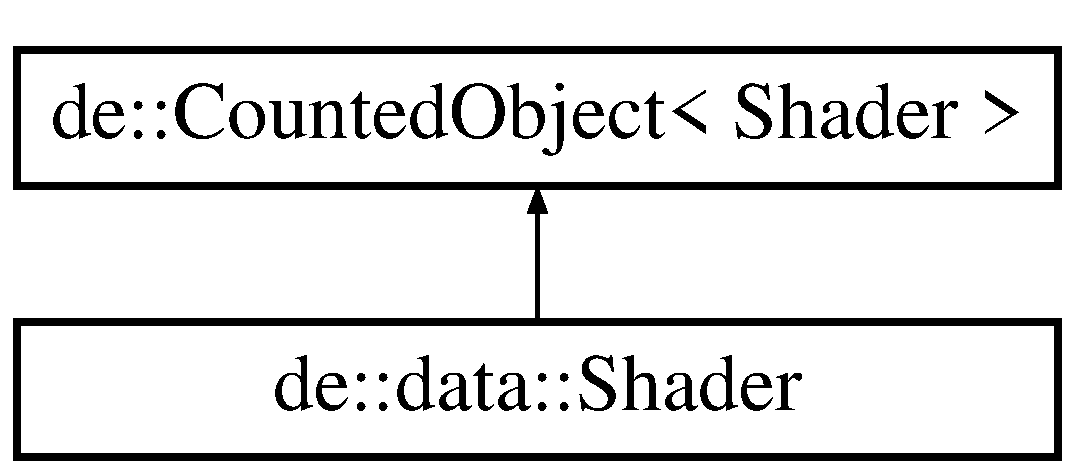
\includegraphics[height=2.000000cm]{classde_1_1data_1_1_shader}
\end{center}
\end{figure}
\subsection*{\-Public \-Types}
\begin{DoxyCompactItemize}
\item 
enum \hyperlink{classde_1_1data_1_1_shader_a51d5bfadf16d2268280b5ffc0ee0ca82}{\-Shader\-Type} \{ {\bfseries \-V\-E\-R\-T\-E\-X} =  \-G\-L\-\_\-\-V\-E\-R\-T\-E\-X\-\_\-\-S\-H\-A\-D\-E\-R, 
{\bfseries \-P\-I\-X\-E\-L} =  \-G\-L\-\_\-\-F\-R\-A\-G\-M\-E\-N\-T\-\_\-\-S\-H\-A\-D\-E\-R, 
{\bfseries \-G\-E\-O\-M\-E\-T\-R\-Y} =  \-G\-L\-\_\-\-G\-E\-O\-M\-E\-T\-R\-Y\-\_\-\-S\-H\-A\-D\-E\-R
 \}
\begin{DoxyCompactList}\small\item\em \-This simply redefine \-Open\-G\-L shader type (avoid to include \-Open\-G\-L stuff) \end{DoxyCompactList}\end{DoxyCompactItemize}
\subsection*{\-Public \-Member \-Functions}
\begin{DoxyCompactItemize}
\item 
\hypertarget{classde_1_1data_1_1_shader_a00c8bf4cd6b0444bd136abae0eb712c3}{
\hyperlink{classde_1_1data_1_1_shader_a00c8bf4cd6b0444bd136abae0eb712c3}{\-Shader} ()}
\label{classde_1_1data_1_1_shader_a00c8bf4cd6b0444bd136abae0eb712c3}

\begin{DoxyCompactList}\small\item\em create an uninitialize shader. \-Init it with init(shadertype); \end{DoxyCompactList}\item 
\hyperlink{classde_1_1data_1_1_shader_ab0bdd894b1d863e0cef81a1abe5cca79}{\-Shader} (\hyperlink{classde_1_1data_1_1_shader_a51d5bfadf16d2268280b5ffc0ee0ca82}{\-Shader\-Type} p\-Type)
\begin{DoxyCompactList}\small\item\em \-Create an empty shader (need to be initialized with some code later) \end{DoxyCompactList}\item 
\hypertarget{classde_1_1data_1_1_shader_af60195244f00992f5d5a5e87a0997bde}{
void {\bfseries init} (\hyperlink{classde_1_1data_1_1_shader_a51d5bfadf16d2268280b5ffc0ee0ca82}{\-Shader\-Type} p\-Type)}
\label{classde_1_1data_1_1_shader_af60195244f00992f5d5a5e87a0997bde}

\item 
\hypertarget{classde_1_1data_1_1_shader_aaeb01a7ded1439a857ba0fb15f387bb3}{
bool {\bfseries is\-Loaded} () const }
\label{classde_1_1data_1_1_shader_aaeb01a7ded1439a857ba0fb15f387bb3}

\item 
\hypertarget{classde_1_1data_1_1_shader_ada143dca593f3d0f094f6fb873d70229}{
\-G\-Luint {\bfseries get\-I\-D} () const }
\label{classde_1_1data_1_1_shader_ada143dca593f3d0f094f6fb873d70229}

\item 
\hypertarget{classde_1_1data_1_1_shader_ab23e02915a3b10549dc50333147d4065}{
bool {\bfseries load\-Shader} (std\-::string p\-Code)}
\label{classde_1_1data_1_1_shader_ab23e02915a3b10549dc50333147d4065}

\item 
\hypertarget{classde_1_1data_1_1_shader_aca7bf7b50373c95750c53e3c4a5b4985}{
bool {\bfseries load\-Shader\-From\-File} (std\-::string p\-Path)}
\label{classde_1_1data_1_1_shader_aca7bf7b50373c95750c53e3c4a5b4985}

\item 
\hypertarget{classde_1_1data_1_1_shader_a0aa3bd18b99a59922dde3ed539d70719}{
std\-::string {\bfseries get\-Shader\-Log} ()}
\label{classde_1_1data_1_1_shader_a0aa3bd18b99a59922dde3ed539d70719}

\item 
\hypertarget{classde_1_1data_1_1_shader_a87def2b6856bbdafa39133cd9cfeb84a}{
void {\bfseries release} ()}
\label{classde_1_1data_1_1_shader_a87def2b6856bbdafa39133cd9cfeb84a}

\end{DoxyCompactItemize}
\subsection*{\-Protected \-Attributes}
\begin{DoxyCompactItemize}
\item 
\hypertarget{classde_1_1data_1_1_shader_a2622c4d3beeaa142cfddbbea08da5567}{
\-G\-Luint {\bfseries m\-Shader\-I\-D}}
\label{classde_1_1data_1_1_shader_a2622c4d3beeaa142cfddbbea08da5567}

\item 
\hypertarget{classde_1_1data_1_1_shader_a11d7c64ba107f21279fc868ebf4277c3}{
bool {\bfseries m\-Is\-Loaded}}
\label{classde_1_1data_1_1_shader_a11d7c64ba107f21279fc868ebf4277c3}

\item 
\hypertarget{classde_1_1data_1_1_shader_a31b88cfe272c86cc17b49db1025aea8b}{
int {\bfseries m\-Type}}
\label{classde_1_1data_1_1_shader_a31b88cfe272c86cc17b49db1025aea8b}

\item 
\hypertarget{classde_1_1data_1_1_shader_a7b9400f1726f29f0be7edabde69bd611}{
std\-::string {\bfseries m\-Error\-Log}}
\label{classde_1_1data_1_1_shader_a7b9400f1726f29f0be7edabde69bd611}

\end{DoxyCompactItemize}


\subsection{\-Detailed \-Description}
\-Encapsulate a shader. \-Simply allow simple loading from file. 

\subsection{\-Constructor \& \-Destructor \-Documentation}
\hypertarget{classde_1_1data_1_1_shader_ab0bdd894b1d863e0cef81a1abe5cca79}{
\index{de\-::data\-::\-Shader@{de\-::data\-::\-Shader}!\-Shader@{\-Shader}}
\index{\-Shader@{\-Shader}!de::data::Shader@{de\-::data\-::\-Shader}}
\subsubsection[{\-Shader}]{\setlength{\rightskip}{0pt plus 5cm}de\-::data\-::\-Shader\-::\-Shader (
\begin{DoxyParamCaption}
\item[{{\bf \-Shader\-Type}}]{p\-Type}
\end{DoxyParamCaption}
)}}
\label{classde_1_1data_1_1_shader_ab0bdd894b1d863e0cef81a1abe5cca79}


\-Create an empty shader (need to be initialized with some code later) 


\begin{DoxyParams}[1]{\-Parameters}
\mbox{\tt in}  & {\em p\-Type} & can be fed an \-Open\-G\-L enum, as \-Shader\-Type is only a redefinition of those. \\
\hline
\end{DoxyParams}


\-The documentation for this class was generated from the following file\-:\begin{DoxyCompactItemize}
\item 
include/data/\-Shader.\-h\end{DoxyCompactItemize}

\hypertarget{classde_1_1component_1_1_transform}{
\section{de\-:\-:component\-:\-:\-Transform \-Class \-Reference}
\label{classde_1_1component_1_1_transform}\index{de\-::component\-::\-Transform@{de\-::component\-::\-Transform}}
}
\-Inheritance diagram for de\-:\-:component\-:\-:\-Transform\-:\begin{figure}[H]
\begin{center}
\leavevmode
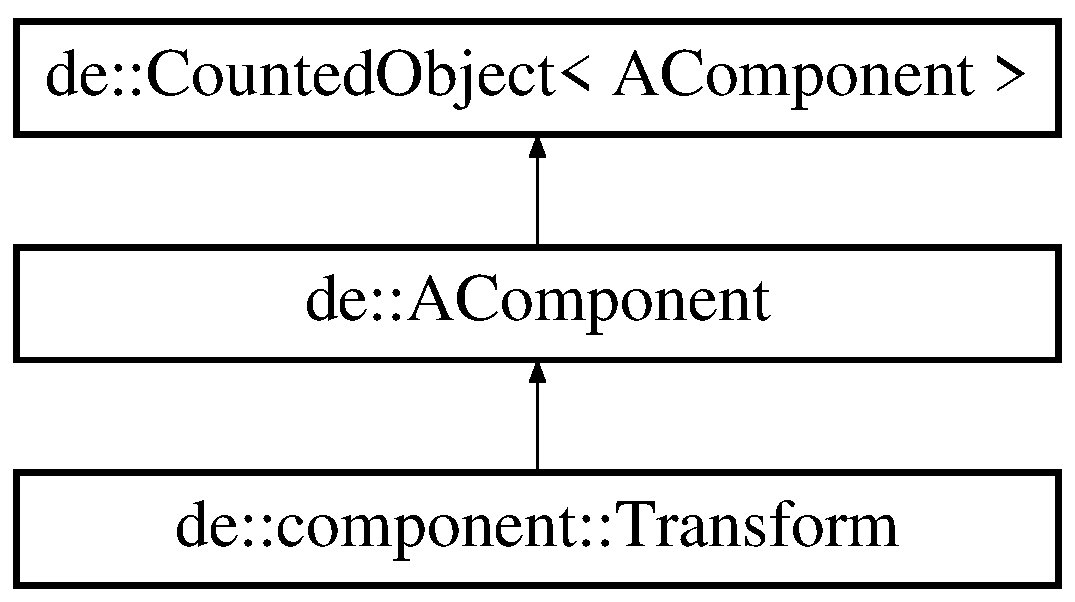
\includegraphics[height=3.000000cm]{classde_1_1component_1_1_transform}
\end{center}
\end{figure}
\subsection*{\-Public \-Member \-Functions}
\begin{DoxyCompactItemize}
\item 
\hypertarget{classde_1_1component_1_1_transform_aa633f78f603b073ded87ce3d76d68c9f}{
void \hyperlink{classde_1_1component_1_1_transform_aa633f78f603b073ded87ce3d76d68c9f}{update} ()}
\label{classde_1_1component_1_1_transform_aa633f78f603b073ded87ce3d76d68c9f}

\begin{DoxyCompactList}\small\item\em called each update \end{DoxyCompactList}\item 
\hypertarget{classde_1_1component_1_1_transform_a21e27db96b4445b5c970633265c13296}{
bool \hyperlink{classde_1_1component_1_1_transform_a21e27db96b4445b5c970633265c13296}{recomputed} () const }
\label{classde_1_1component_1_1_transform_a21e27db96b4445b5c970633265c13296}

\begin{DoxyCompactList}\small\item\em this return true if the transform was recomputed this frame. \-As \hyperlink{classde_1_1component_1_1_transform}{\-Transform} is always the first to be updated, this allow other component to know if the game\-Object was moved or changed in any manner \end{DoxyCompactList}\item 
\hypertarget{classde_1_1component_1_1_transform_a01da3717d44a091953ce85e5ca6e3a4f}{
glm\-::mat4 \hyperlink{classde_1_1component_1_1_transform_a01da3717d44a091953ce85e5ca6e3a4f}{matrix} () const }
\label{classde_1_1component_1_1_transform_a01da3717d44a091953ce85e5ca6e3a4f}

\begin{DoxyCompactList}\small\item\em return the matrix combining all transformation \end{DoxyCompactList}\end{DoxyCompactItemize}
\subsection*{\-Protected \-Attributes}
\begin{DoxyCompactItemize}
\item 
\hypertarget{classde_1_1component_1_1_transform_a1a0d80838c02e57bc271516572784ee4}{
glm\-::vec3 {\bfseries m\-Position}}
\label{classde_1_1component_1_1_transform_a1a0d80838c02e57bc271516572784ee4}

\item 
\hypertarget{classde_1_1component_1_1_transform_a791f59c644c4af4d31ac000a61eb4716}{
glm\-::vec3 {\bfseries m\-Local\-Position}}
\label{classde_1_1component_1_1_transform_a791f59c644c4af4d31ac000a61eb4716}

\item 
\hypertarget{classde_1_1component_1_1_transform_acde4ad08f2bb859b01885b6133f43e53}{
glm\-::quat {\bfseries m\-Rotation}}
\label{classde_1_1component_1_1_transform_acde4ad08f2bb859b01885b6133f43e53}

\item 
\hypertarget{classde_1_1component_1_1_transform_ac4a7eecdbe7457b3331e26a4c9e4939b}{
glm\-::quat {\bfseries m\-Local\-Rotation}}
\label{classde_1_1component_1_1_transform_ac4a7eecdbe7457b3331e26a4c9e4939b}

\item 
\hypertarget{classde_1_1component_1_1_transform_a64bdb4a44b50f610c6fb34b13d74f65f}{
glm\-::vec3 {\bfseries m\-Local\-Scale}}
\label{classde_1_1component_1_1_transform_a64bdb4a44b50f610c6fb34b13d74f65f}

\item 
\hypertarget{classde_1_1component_1_1_transform_a46f0487729770e66da59ddc8df4fe02e}{
glm\-::mat4x4 {\bfseries m\-Matrix}}
\label{classde_1_1component_1_1_transform_a46f0487729770e66da59ddc8df4fe02e}

\item 
\hypertarget{classde_1_1component_1_1_transform_a8ec6eb4a7ec9b73e08f1b6e5bf7c1299}{
bool {\bfseries m\-Changed}}
\label{classde_1_1component_1_1_transform_a8ec6eb4a7ec9b73e08f1b6e5bf7c1299}

\item 
\hypertarget{classde_1_1component_1_1_transform_a8d1518abb22163f75fff74b98b814d19}{
bool {\bfseries m\-Recomputed}}
\label{classde_1_1component_1_1_transform_a8d1518abb22163f75fff74b98b814d19}

\end{DoxyCompactItemize}


\-The documentation for this class was generated from the following file\-:\begin{DoxyCompactItemize}
\item 
include/component/\-Transform.\-h\end{DoxyCompactItemize}

\printindex
\end{document}
